\section{Simulation}


There are two different, though overlapping, areas in our current simulation 
effort. One is focused on validating design decisions for the upgraded 
detector, the other on building a modern simulation system that can be used 
for the life of the {\tt CLAS12} program. The former has two components: (1) a 
parametric Monte Carlo that can estimate the resolution for charged particle 
tracking and (2) a full GEANT3 system that depends on the code base that has 
been developed for the current {\tt CLAS} detector, modified to reflect the 
new design, including reconstruction. The latter is an entirely new 
GEANT4-based, object-oriented design.

\vskip 0.5cm

\noindent
\underline{Parametric Monte Carlo}

One of the fundamental algorithmic challenges in the design of {\tt CLAS12} 
is the problem of track reconstruction in a non-uniform magnetic field.  Not 
only does the torus produce an inhomogeneous field in the tracking volume, 
but charged particles emerging from the solenoid must be tracked as they 
traverse the fringe field of that magnet. Since no analytic form for the 
particle trajectories exist, they must be calculated by "swimming" the
particles numerically through a map of the magnetic field. Track fitting 
then becomes very expensive in terms of cpu time. One way to finesse the 
problem is to linearize it by parameterizing the trajectory as small deviations 
from a reference trajectory. The reference trajectory must come from a 
``swim'', but subsequent ``trial'' trajectories, with different starting 
parameters (momentum, direction), can be computed by a simple matrix 
inversion. Position resolution is put in at a set of idealized detector 
planes. It is also possible to incorporate multiple Coulomb scattering in 
this model. This technique has already been used to estimate momenta 
resolution for {\tt CLAS12}. Results appear in other sections of this 
document.  The method cannot give information on some things, such as the 
effect of accidentals, track reconstruction efficiency or confusion due to 
overlapping tracks.

\vskip 0.5cm

\noindent
\underline{{\tt CLAS} Software with {\tt CLAS12} Geometry}

The current {\tt CLAS} system consists of over a half a million lines of 
FORTRAN, C and C++ code contained in about 2,500 source code files. It 
represents a large investment by the {\tt CLAS} collaboration over many 
years. {\tt CLAS}, with its toroidal magnetic field also presents the 
difficulty of tracking in a non-homogeneous fields and that problem has 
been solved in this body of code. Recently, the geometry of crucial detector 
elements was changed to reflect the {\tt CLAS12} design, both in simulation 
and in reconstruction. The resulting system can now do a full GEANT3-based 
simulation and reconstruction of {\tt CLAS12} events, in particular charged 
particle tracking in the forward drift chambers. Studies using this system 
have been carried out to verify momentum resolution results from the 
parametric Monte Carlo and to estimate the effect of accidental M{\o}ller 
scattering background on track reconstruction. More of the details of the 
detector subsystems and beam line components of the upgraded configuration 
are being added to extend the range of these and similar studies.

\vskip 0.5cm

\subsection{Geant4 Object-Oriented Detector Simulation}

The Geant4 simulation software for CLAS12 is called {\tt gemc} ({\tt GE}ant4 {\tt M}onte{\tt C}arlo).
The parameters that define the simulation (i.e. geometry, sensitivity, magnetic fields, output banks, etc)
are stored in an external database and used at run-time in STL (c++ Standard Template Library) objects.
The database currently in use is the {\tt mysql} database. Other options (e.g. XML) are also available for consideration.

\vskip 0.5cm

\underline{Geometry}
\vskip 0.5cm

\noindent
The Geant4 volumes are defined as follows:

\noindent
\begin{itemize}
\item Shapes, dimensions. Boolean operations of shapes.
\item Material, Magnetic Field, Visual attributes, Identity, Sensitivity and Hit Process.
\item Placement(s) in space: position, rotation, copy number.
\end{itemize}

\noindent
These parameters are stored in mysql tables, one table per detector (i.e. HTCC, EC, DC, etc).
At run time, gemc reads a {\tt gcard}, an XML file that specifies which detector to include in the simulation, including
possible tilts and displacements from the original positions. An example of {\tt gcard} syntax:

\footnotesize
\begin{verbatim}
<sqltable name="LH2target"/>   - Includes the Liquid Hidrogen Target
<sqltable name="BST"/>         - Includes the Barrel Silicon Vertex Tracker
<sqltable name="FST"/>         - Includes the Forward Silicon Vertex Tracker
<sqltable name="CTOF"/>        - Includes the Central TOF
<sqltable name="beamline"/>    - Includes the beamline
<sqltable name="DC"/>          - Includes the Drift Chambers

<detector name="BST">
 <position x="0*cm"  y="0.1*cm" z="0*cm" /> - Displaces the BST by 1 mm in the Y axis
 <rotation x="1*deg" y="0*deg"  z="0*deg"/> - Titls the BST by 1 degree around the X axis
</detector>
\end{verbatim}
\normalsize

\underline{CLAS12 Geometry Implementation}
\vskip 0.5cm

\noindent
Particular attention is paid in reproducing in gemc the design of each detector with as much accuracy and
as many details as reasonably achievable.
In Fig.~\ref{fig:svt} the SVT Geant4 representation is shown, while in Fig.~\ref{fig:central} is shown
the Geant4 implementation of the various central detectors.


\vskip 1cm
\begin{figure}[h]
\begin{center}
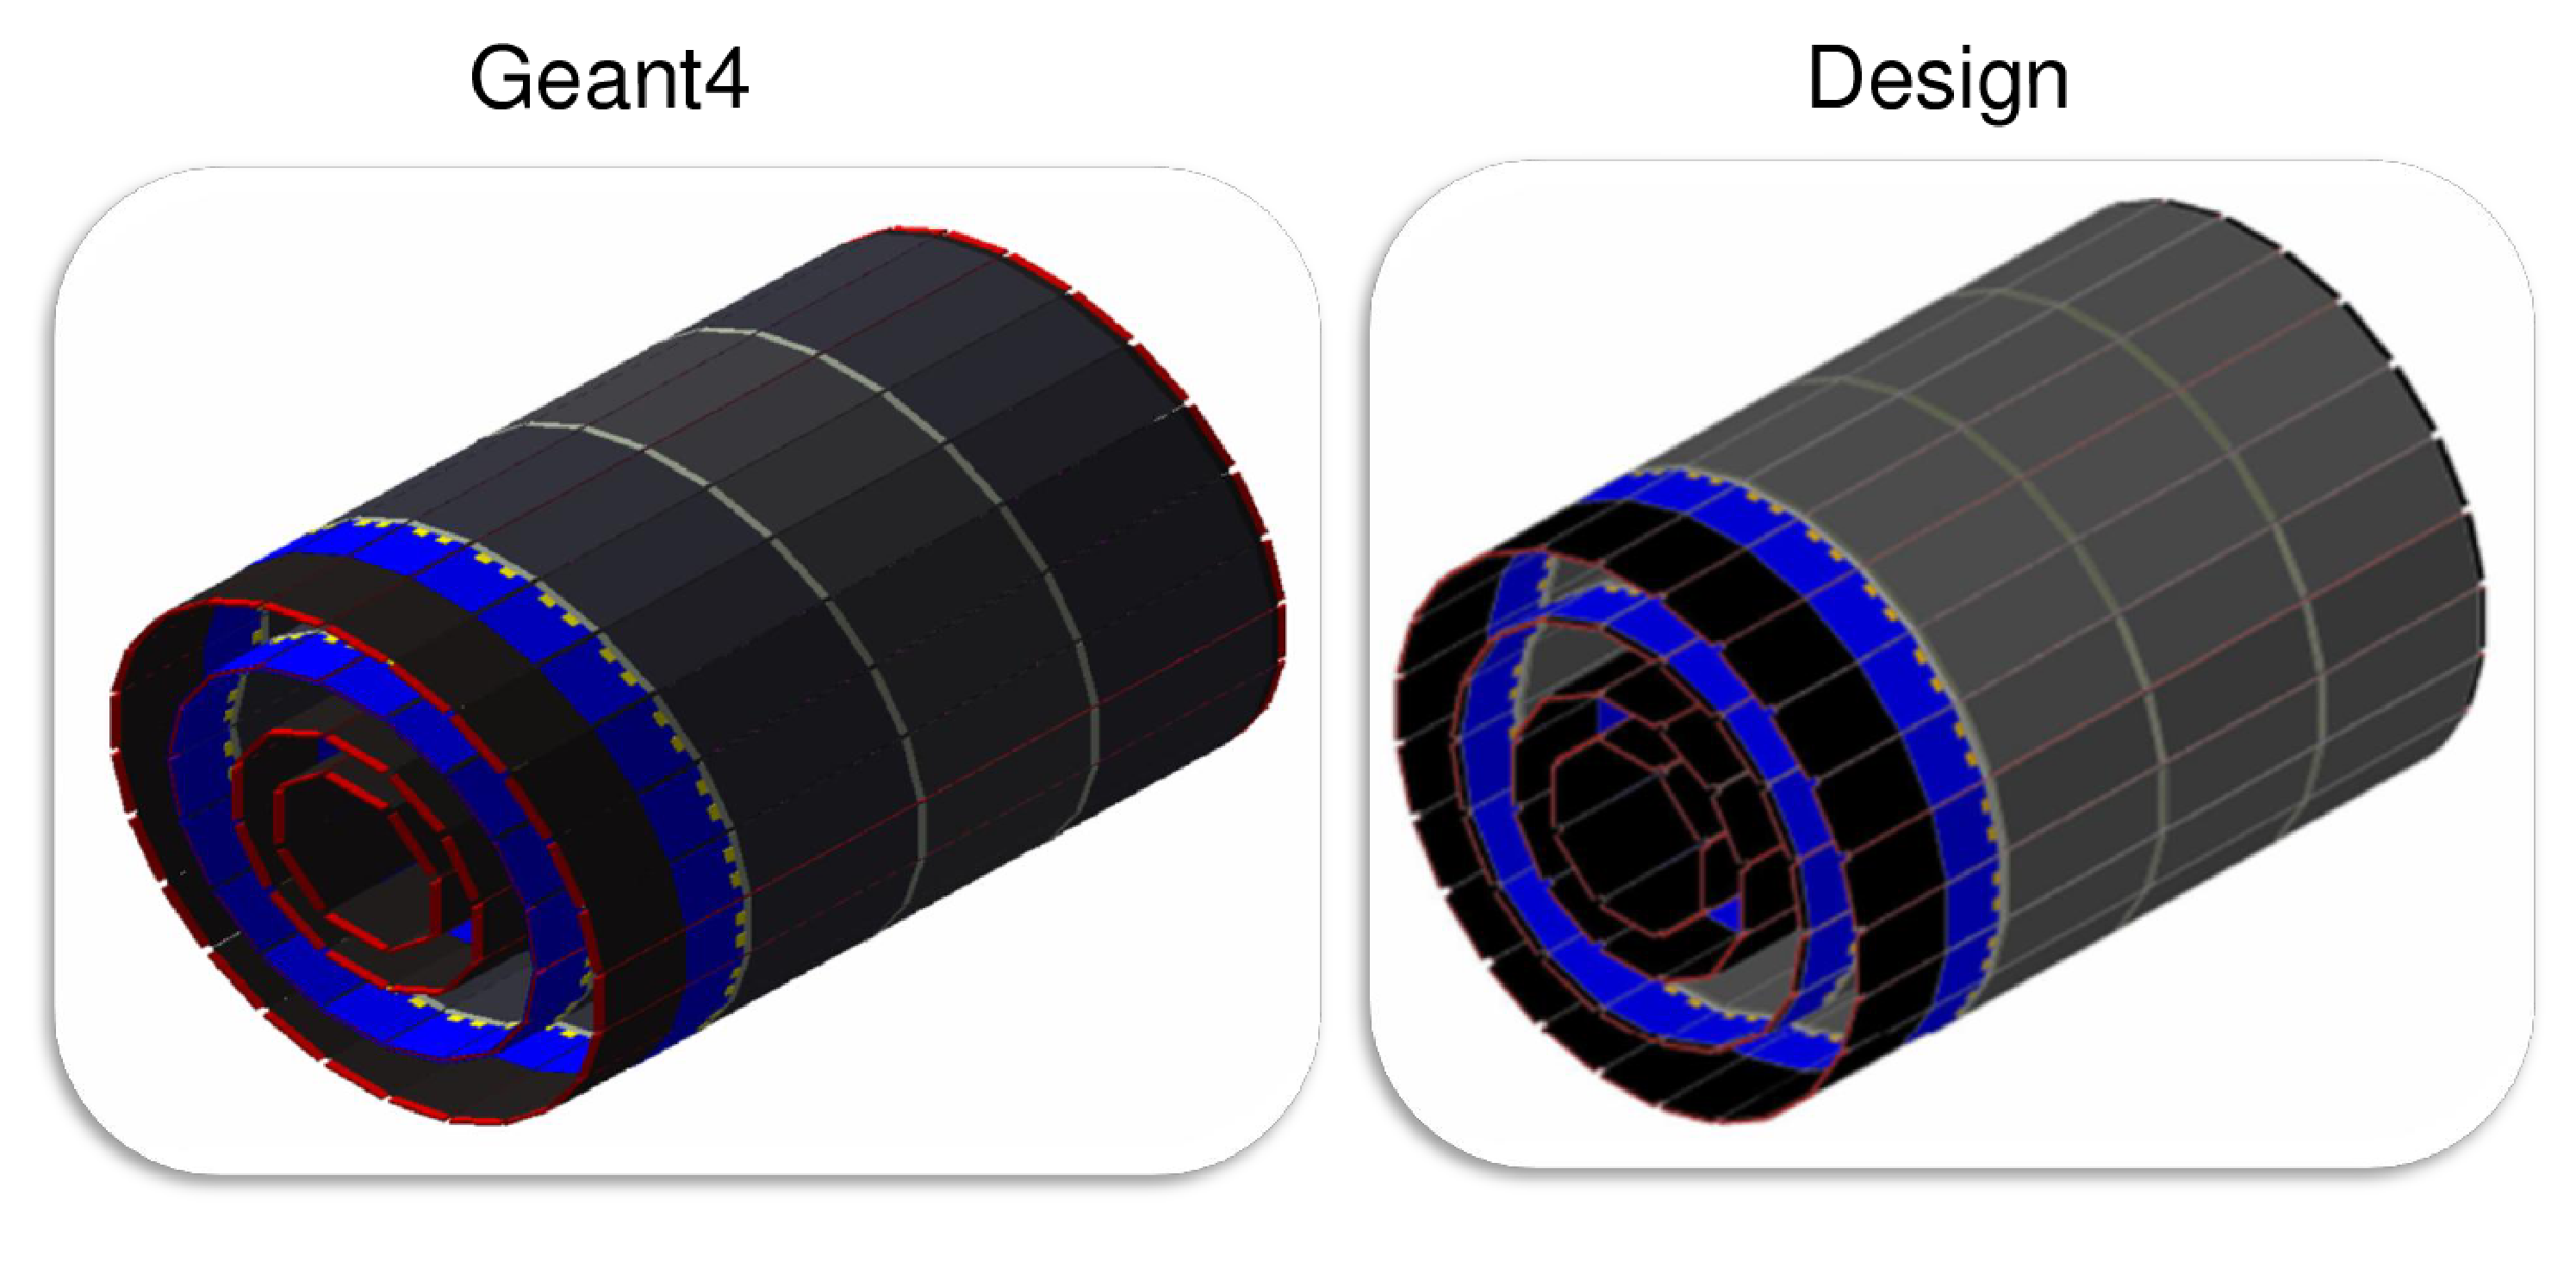
\epsfig{file=Simulation/bst.eps,width=15.0cm,height=7cm}
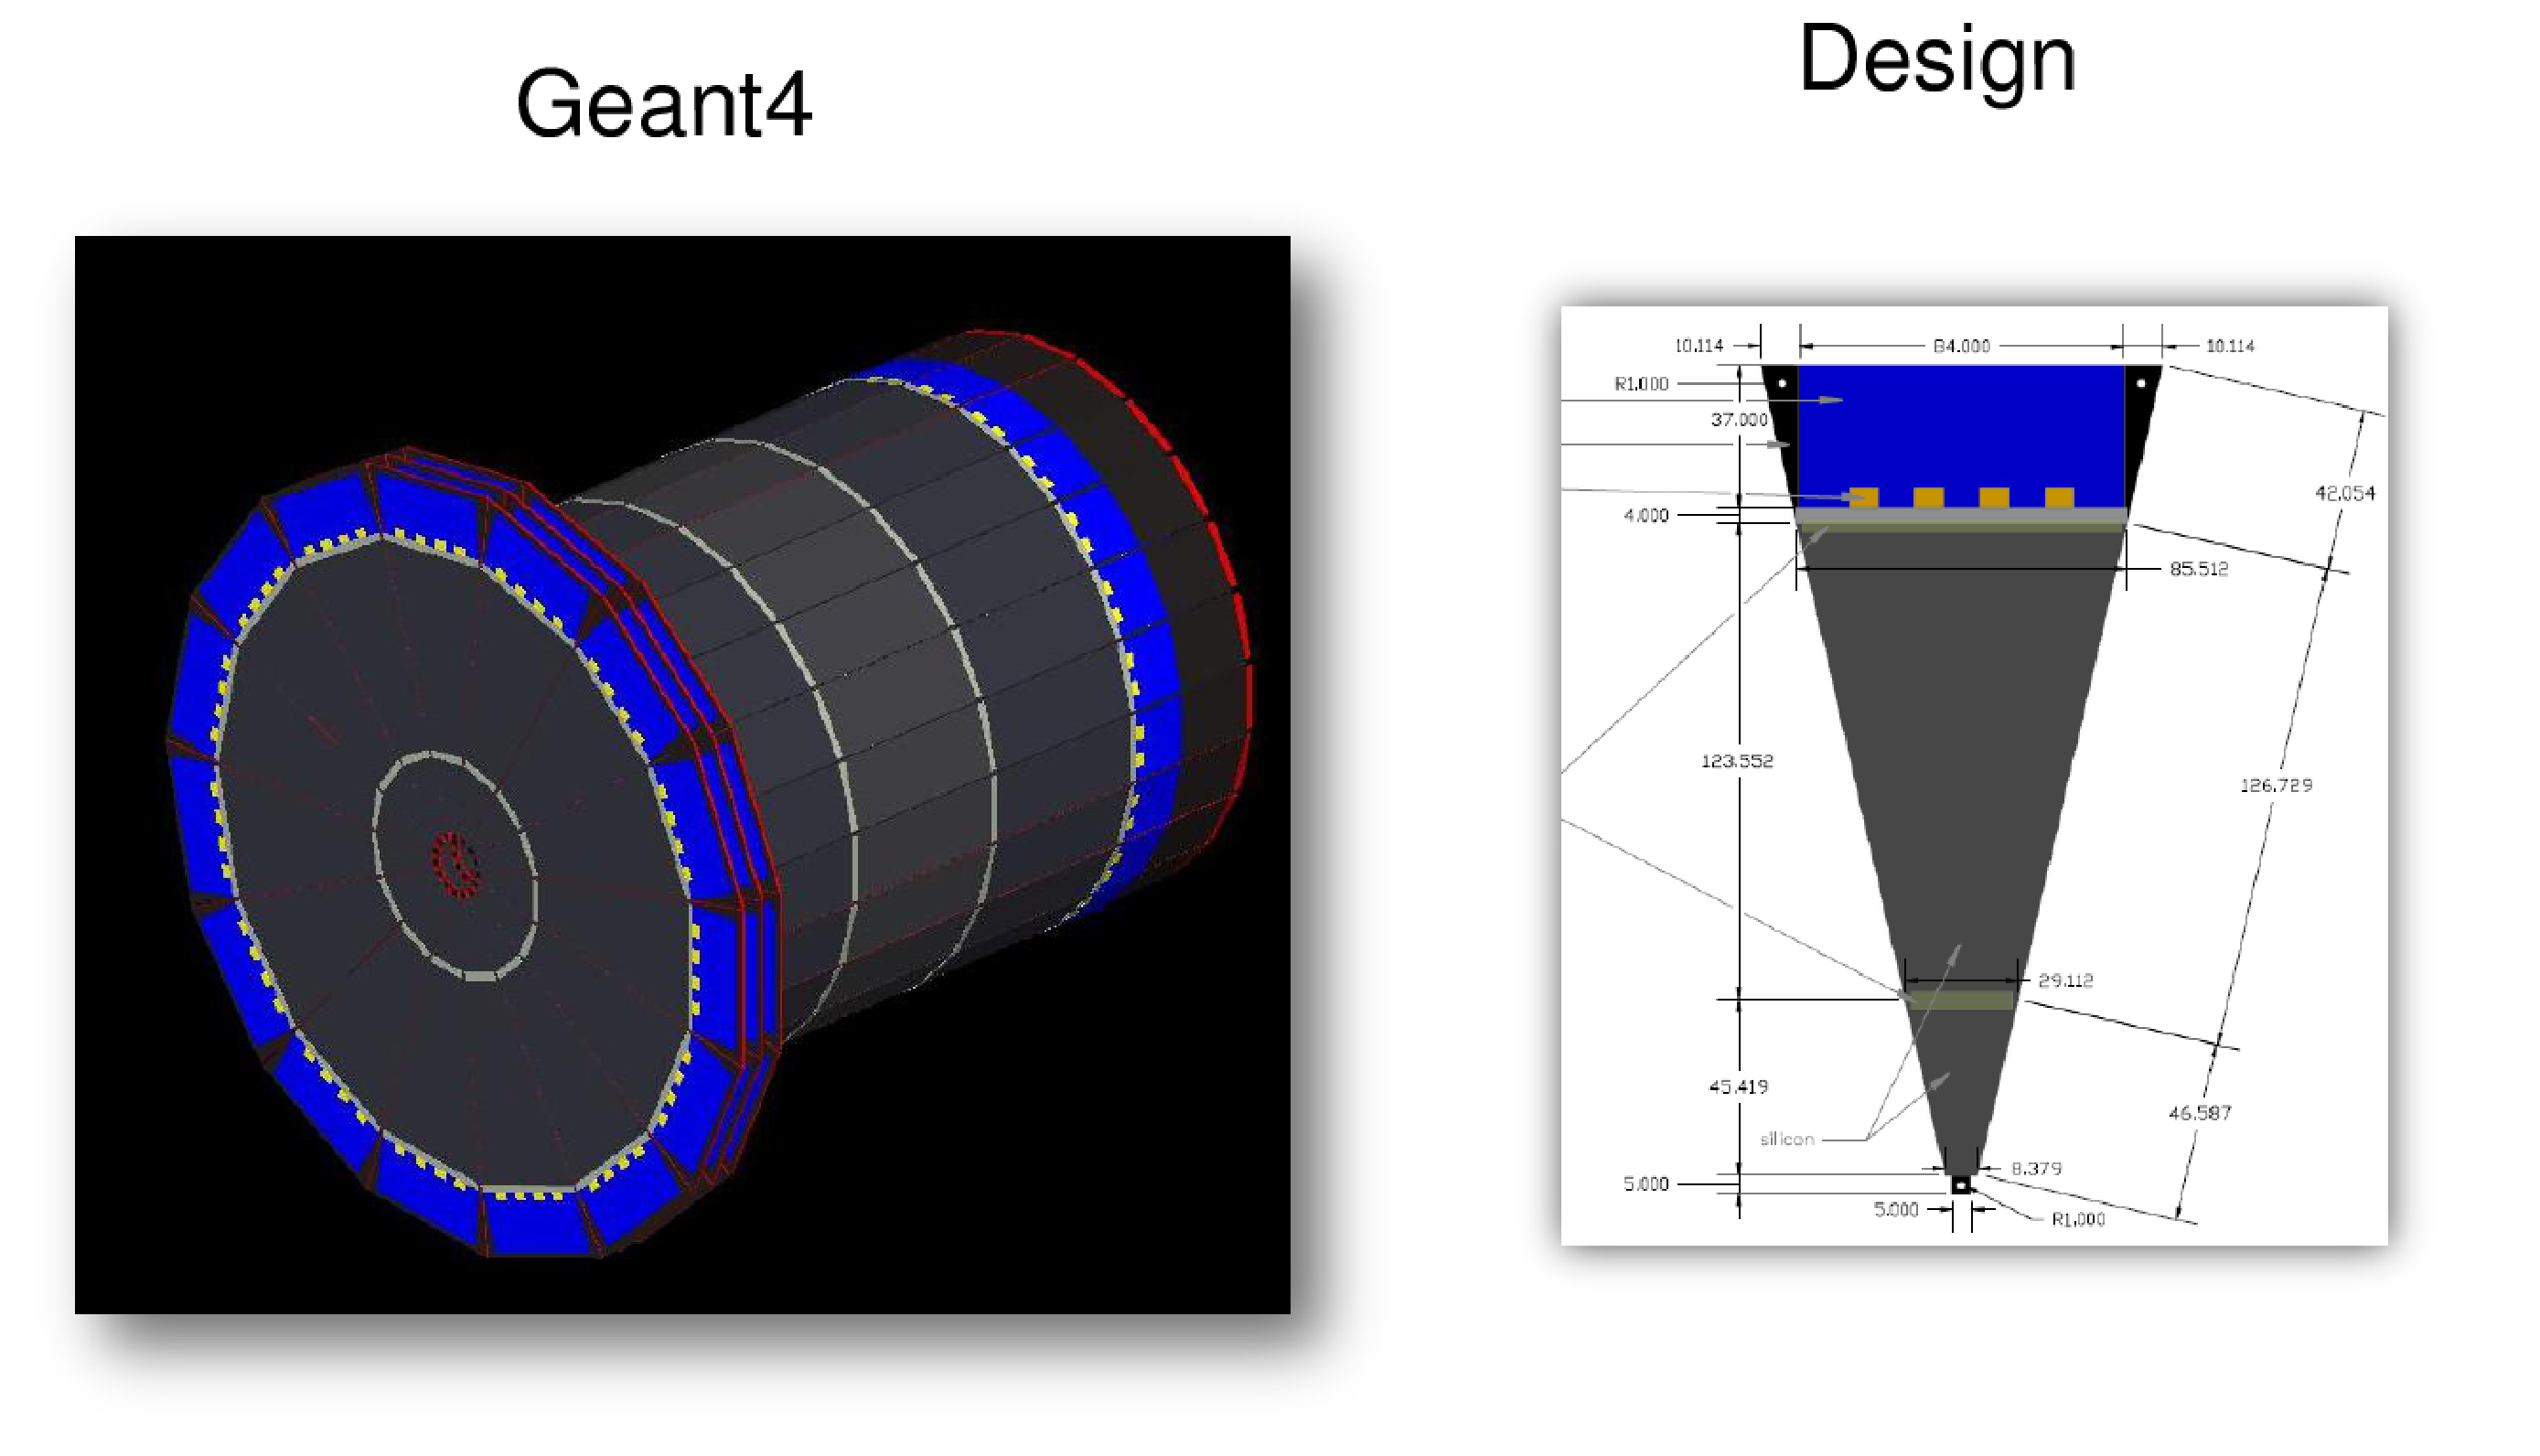
\epsfig{file=Simulation/svt.eps,width=15.0cm,height=7cm}
\caption{\small{The Silicon Vertex Tracker in Geant4. Upper left: the gemc BST.
               Upper right: the CAD model. Lower Left: the complete gemc implementation of
               the BST+FST. Lower right: an FST module. All components (including supports,
               wirebonds and chips) and dimensions in gemc reproduce exactly the design. }}
\label{fig:svt}
\end{center}
\end{figure}
\clearpage\newpage
\begin{figure}[h]
\begin{center}
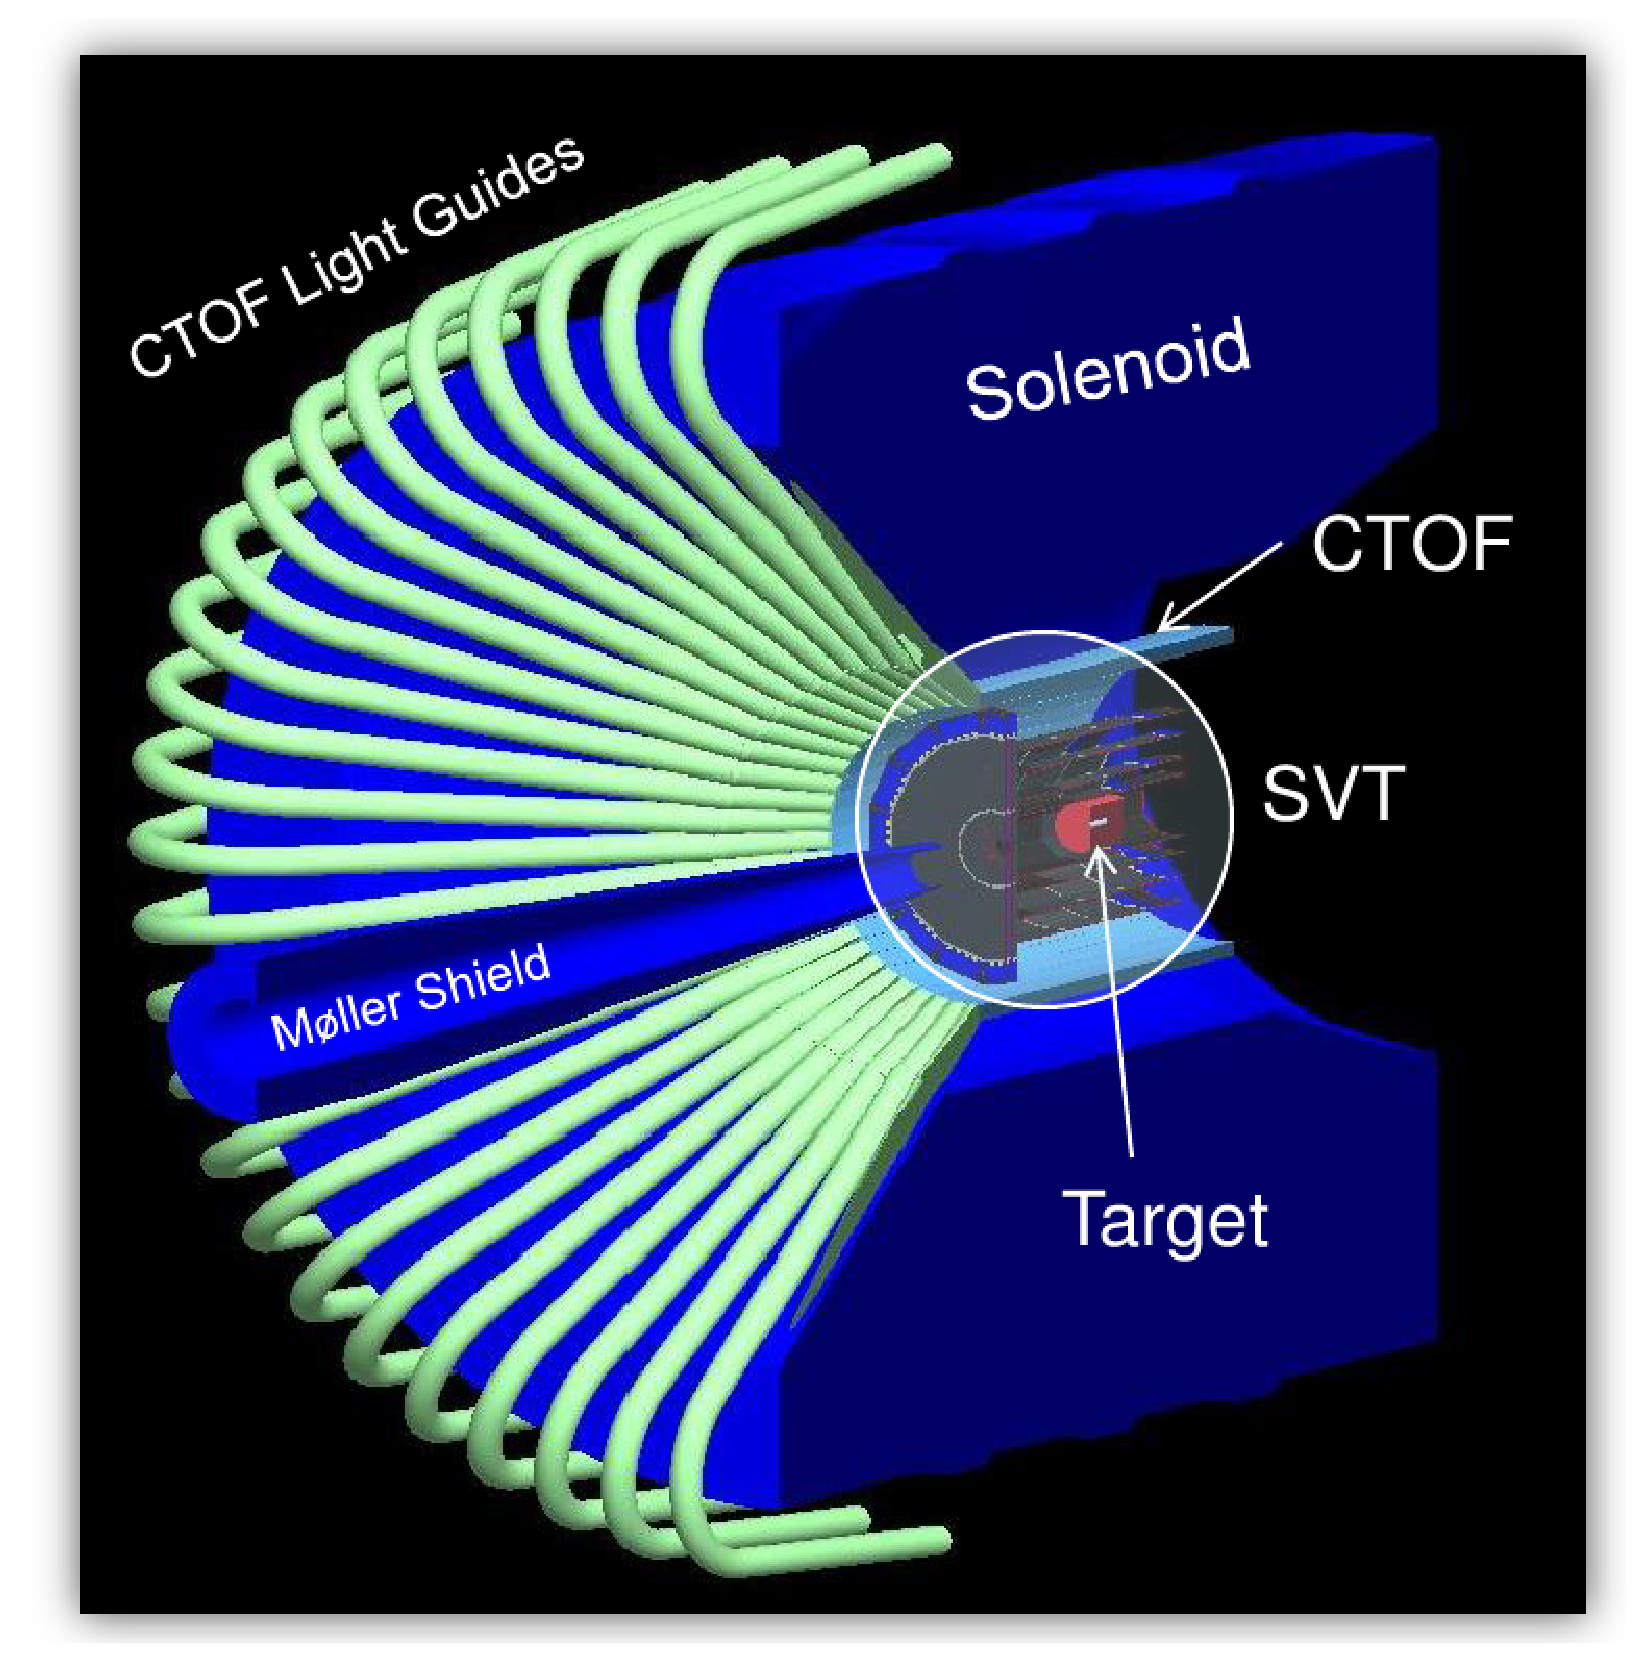
\epsfig{file=Simulation/central.eps,width=16.0cm,height=16cm}
\caption{\small{The CLAS12 Central Detector. The Target (white) is at the CLAS12 center,
               surrounded by the Scattering Chambers (red). The BST and FST constitute the
               Silicon Vertex Tracker. The CTOF paddles (cyan) are connected to light guides
               (light green) that wrap around the Solenoid (blue). The Moeller Shield is also
               visible (blue).}}
\label{fig:central}
\end{center}
\end{figure}
\clearpage\newpage


\underline{Generator}
\vskip 0.5cm

\noindent
In gemc there are two ways to define the primary generator:
\begin{itemize}
\item[1)] {\tt gemc internal generator} (command line or {\tt gcard}): with this method the user
defines the primary particle type, momentum range, vertex range. Example:

\footnotesize
\begin{verbatim}
BEAM_P="proton, 0.8*GeV, 80*deg, 10*deg"
SPREAD_P="0.2*GeV, 40*deg, 40*deg"

BEAM_V="(0.0, 0.0, 0.0)cm"
SPREAD_V="(0.1, 0.1, 2.5)cm"

results in:

Primary Particle:  Proton
momentum: 800 +- 200 MeV
theta: 80 +- 40 deg
Phi: 10 +- 40 deg
Vertex: ( +- 1 mm , +- 1mm +- 2.5cm) 

\end{verbatim}
\normalsize

\item[2)] {\tt external input file}: with this method the user defines (command line or {\tt gcard}) the format
of the input file and the file name. Example:
\footnotesize
\begin{verbatim}
INPUT_GEN_FILE="LUND, dvcs.dat"  - LUND file format, filename:  dvcs.dat
\end{verbatim}
\normalsize 
\end{itemize}

The various file formats are registered in gemc by a {\it factory method}, that allows to derive
new formats from the gemc c++ pure virtual methods defined for the input, and to choose
the desired format at run-time.

\vskip 0.5cm
In addition to the primary particles, an additional {\it luminosity beam} can be defined to add realistic background
to the simulation. The user defines  (command line or {\tt gcard}) the beam particle type,
the number of beam particles per event, and the time structure of the beam. Example:

\footnotesize
\begin{verbatim}
LUMI_P="e-, 11*GeV, 0, 0"         Beam Particles: 11 GeV e- along z-axis
LUMI_V="(0, 0, -10)cm"            Beam vertex is at z=-10 cm
LUMI_EVENT="60000, 124*ns, 2*ns"  60,000 particles per event, spread in 124 ns, 2ns per bunch

\end{verbatim}
\normalsize

\vskip 0.5cm
\underline{Hit Definition}
\vskip 0.5cm

\noindent
The gemc hit definition is illustrated in Fig.~\ref{fig:hit_def}. A {\tt Time Window} (TW)
is associated with each sensitive detector. In the same detector element, tracks within
the TW constitute one hit, while tracks separated in time by more than the TW form two 
separate hits.

\vskip 1cm
\begin{figure}[h]
\begin{center}
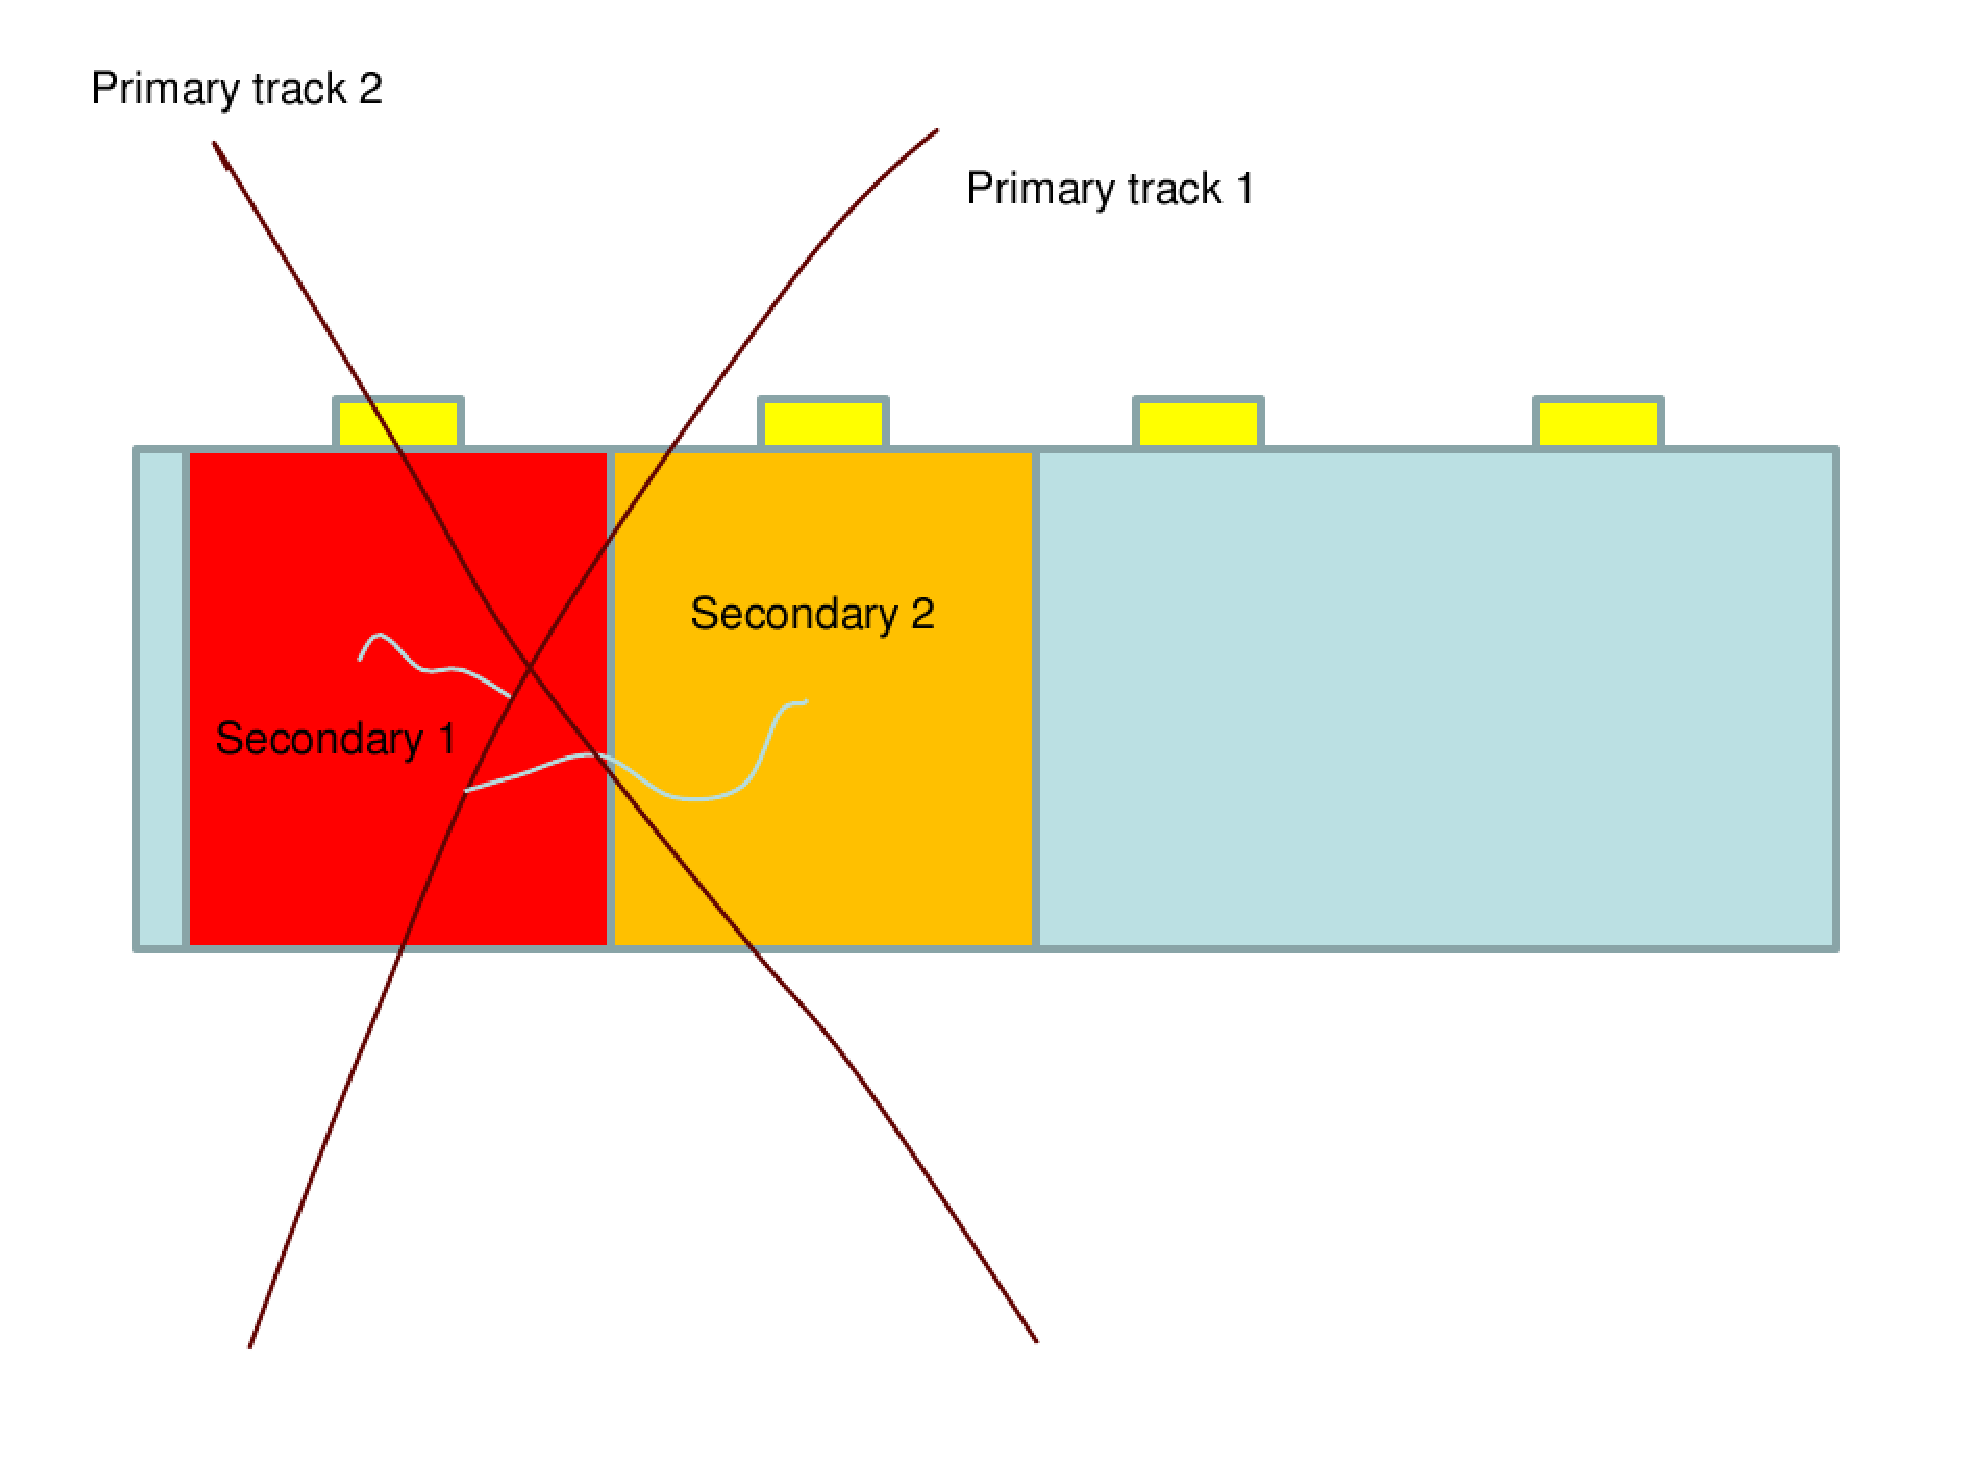
\epsfig{file=Simulation/hit.eps, width=15.0cm,height=12cm}
\caption{\small{Hit Definition Illustration: In the picture two different detector elements 
               are shown in different colors (red and light brown). All tracks within the same TW
               and the same cell constitute one hit for that cell.
               If any track has enough time separation from an existing hit, it will form another, separate hit.  }}
\label{fig:hit_def}
\end{center}
\end{figure}
\clearpage\newpage


\vskip 1.0cm
\underline{Hit Process Factory}
\vskip 0.5cm

\noindent
Each detector has a custom Hit Process Routine (HPR) associated with it. The gemc HPR pure virtual method is
used to derived all the detectors routines, and all HPRs are registered at run-time
by a factory method.

The input to all HPRs is a {\tt gemc hit}. This stores, for each step in the hit, the following informations:
\vskip 0.5cm
\begin{itemize}
\item Hit Position (global coordinates)
\item Hit Position (relative to the volume in which the step occurs)
\item Deposited energy
\item Time of the hit
\item Momentum of the Track
\item Energy of the track
\item Primary Vertex of track
\item particle ID
\item G4Track ID
\item Identity
\item Detector Hit
\item Mother particle ID
\item Mother G4Track ID
\item Mother Primary Vertex of track
\item Energy Threshold of the sensitive detector
\end{itemize}

\vskip 0.5cm

Each HPR processes the {\tt gemc hit} and produces STL vectors of double (raw informations)
and integers (digitized informations). Each vector correspond to a mysql entry in the bank table
corresponding to the HPR. 

\clearpage\newpage
\vskip 2cm
Below are three examples of such database entries.

\begin{itemize}
\item A partial list of variables used to store ''raw`` informations, usually common to all detectors:
\footnotesize
\begin{verbatim}
        name      index       comment
        ETot        1     Total Energy Deposited
        <x>         2     Average x position
        <y>         3     Average y position
        <z>         4     Average z position
        <t>         8     Average time
        pid         9     Particle ID
         E         13     Energy of the track at the entrance point
\end{verbatim}
\normalsize

\vskip 1cm
\item A partial list of variables used to store DC informations:
\footnotesize
\begin{verbatim}
        name          index           comment
         LR            18       Left/Right: -1 (right) if the track is below the wire
        doca           19       distance of closest approach
        sdoca          20       smeared doca
        time1          21       doca / (50 um/ns)
       stime1          22       sdoca / (50 um/ns)
       sector          23       CLAS12 Sector
     superlayer        24       DC Superlayer
       layer           25       DC Layer
        wire           26       DC Wire
\end{verbatim}
\normalsize

\vskip 1cm
\item A partial list of variables used to store BST informations:
\footnotesize
\begin{verbatim}
        name      index        comment
       layer       20         BST layer
      sector       21         BST sector
       strip       22         BST strip
\end{verbatim}
\normalsize
\end{itemize}
\clearpage\newpage



\vskip 1.0cm
\underline{Elements Identity}
\vskip 0.5cm
\noindent In order to correctly identify and process the correct detector element at run time, a class {\tt identifier} is used.
The following scenarios can happen:

\begin{itemize}


\item[1)] For detectors where each element corresponds to a unique volume, the identifier remains unchanged.
An example is the CTOF:
\footnotesize
\begin{verbatim}
element          identifier
paddle 4              4
paddle 16            16
\end{verbatim}
\normalsize



\item[2)] For detectors where each element corresponds to a unique volume that is copied, the identifier copy number is
determined at run time.
An example is the OTOF, where each sector is copied:
\footnotesize
\begin{verbatim}
     element           identifier: sector copy is determined at run time.
paddle 4,  sector 3                           4, 3
paddle 16, sector 5                          16, 5
\end{verbatim}
\normalsize


\item[3)] For detectors where different elements correspond to the same volume, the identifier is processed
at run-time by the identifier method of the Hit Process Routines described above. For example, in the Drift Chambers implementation
the single cells are not geant4 volumes (due to the fact that there are too many of them).
The sensitive volumes are instead layers of gas. At run-time, the cell is identified by the HPR
based on the track position in each layer:
\footnotesize
\begin{verbatim}
           element                identifier: sector, wire are determined at run-time
wire 52, layer 3, SL 2, sector 4                      52, 3, 2, 4
wire 87, layer 4, SL 5, sector 1                      87, 4, 5, 1
\end{verbatim}
\normalsize

\end{itemize}


\clearpage\newpage

\vskip 1.0cm
\underline{Output}
\vskip 0.5cm

\noindent
The file formats for the simulation output stream are registered in gemc by a factory method. New files types
can be derived from the c++ pure virtual methods defined in gemc. The main registered formats, selectable at run-time, are:

\begin{itemize}
\item txt: readable from any editor or shell. Bank names, variables are printed out.
\item EVIO: this is the format used by the CODA system, and unanimously chosen to be the
default format for the output stream. Banks and variables are identified by integers (tag and num)
defined in the mysql tables.
\end{itemize}

The EVIO output can be viewed with the utility evio2xml, that outputs event in XML format.
As illustration, an example of a EVIO event dumped with evio2xml:
\footnotesize
\begin{verbatim}

<event_n>   3  </event_n>

<particle_generator>
 <generated_particle_1>
   2212 1.0+03 0.0 1.7321e+03  - particle id, 3-momentum
   0.0  0.0  0.0               - vertex
 </generated_particle_1>
</particle_generator>

<DC>    DC has 3 hits, so each variables has 3 entries
  <sector>      2              2              2   </sector>
  <SuperLayer>  3              3              3   </SuperLayer>
  <Layer>       1              2              3   </Layer>
  <Wire>       71             70             71   </Wire>
  <Edep>   1.4498e-04   1.1808e-03   1.0493e-03   </Edep>
</DC>
\end{verbatim}
\normalsize

\vskip 0.5cm
\underline{Doxygen Documentation}
\vskip 0.5cm
The c++ code is documented with doxygen. The documentation can be found here:
\begin{verbatim}
        http://clasweb.jlab.org/clas12/gemc_doxygen
\end{verbatim}

